\section{Pozorování latentního prostoru}
\label{sec:vae_model_latent_space_observation}

\begin{figure}[H]
    \centering
    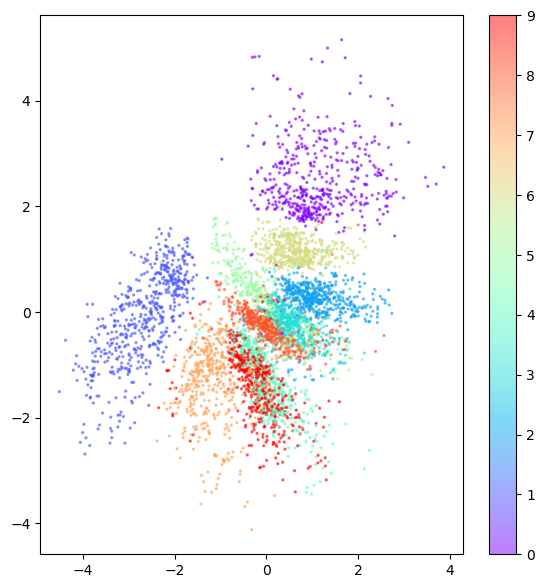
\includegraphics[width=\textwidth]{figures/latent_space_200_epochs.png}
    \caption{Latentní prostor naučeného modelu variačního autoenkodéru. Barvy reprezentují jednotlivé třídy MNIST datasetu, tedy číslice $0$ - $9$. }
\end{figure}

\begin{figure}[H]
    \centering
    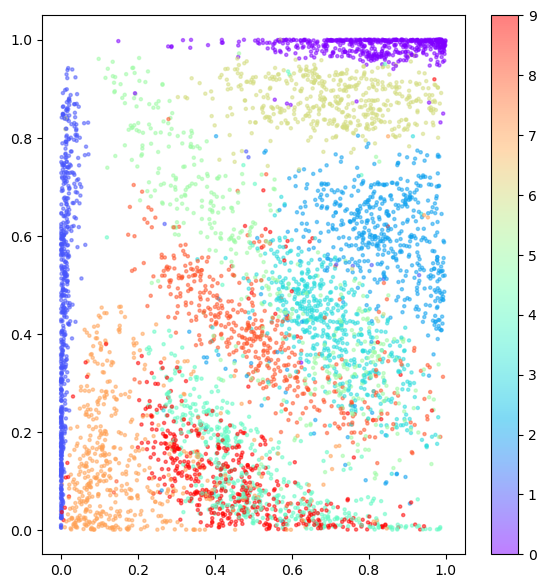
\includegraphics[width=\textwidth]{figures/vae_latent_space_p_values.png}
    \caption{Latentní prostor naučeného modelu variačního autoenkodéru. Barvy reprezentují jednotlivé třídy MNIST datasetu, tedy číslice $0$ - $9$. }
\end{figure}